\documentclass[letterpaper,twocolumn,10pt]{article}
\usepackage{usenix,endnotes,multirow}
\usepackage{cleveref,amsmath,chngcntr}
\usepackage{framed}
\usepackage{multicol,tabularx}
\usepackage{textcomp} % for tilde
\usepackage{paralist} % for in-paragraph lists

% For drawing FSMs
\usepackage{tikz}
\usetikzlibrary{arrows,automata}

% Used for code snippets
\usepackage{listings,courier}

% Used for changing the spacing after the title, sections, and subsections.
\usepackage{titlesec,titling}

% Make text in figure captions small
\usepackage{caption3} % load caption package kernel first
\DeclareCaptionOption{parskip}[]{} % disable "parskip" caption option
\usepackage[small]{caption}
%\usepackage{subfigure,epsfig}
%\captionsetup*[subfigure]{position=bottom}
\usepackage{subcaption}
\captionsetup{compatibility=false}
\usepackage{epsfig}

% Make sure that figure numbers are continuous through the document
%\counterwithout{figure}{section}
%\counterwithout{figure}{subsection}

% Settings on code listings.
\lstset{language=C,
		xleftmargin=0pt,
		xrightmargin=0pt,
		framexbottommargin=0pt,
        framextopmargin=0pt,
        framesep=0pt}

% Modify spacing before/after title, sections, and subsections.
\setlength{\droptitle}{-3em} 
\posttitle{\par\end{center}\vspace{-1.5em}}


\titlespacing\section{0pt}{5pt plus 4pt minus 2pt}{5pt plus 2pt minus 2pt}        
\titlespacing\subsection{0pt}{5pt plus 4pt minus 2pt}{5pt plus 2pt minus 2pt}   

\usepackage{enumitem}
\setenumerate{itemsep=2pt,topsep=2pt,parsep=0pt,partopsep=0pt}
%
%% Compressed enumerations
%\newenvironment{enumerate*}%
%  {\begin{enumerate}[topsep=0pt]%
%    \setlength{\itemsep}{2pt}%
%    \setlength{\topsep}{0pt}%
%    \setlength{\partopsep}{0pt}%
%    \setlength{\parsep}{0pt}%	
%    \setlength{\parskip}{0pt}}%
%  {\end{enumerate}}

% Compressed bibliograpgy
\let\ORIGbibliography\bibliography
\renewcommand{\bibliography}[1]{{\footnotesize \ORIGbibliography{#1}}}

% Add a horizontal rule above captions, and make captions closer to their figures
\DeclareCaptionFormat{ruled_caption}{#1#2#3\hrulefill}
\DeclareCaptionFormat{unruled_caption}{#3}
\captionsetup[figure]{format=ruled_caption}
\captionsetup[subfigure]{format=unruled_caption}
\let\ORIGcaption\caption
\renewcommand{\caption}[2][\compressedcaption]{%
\def\compressedcaption{#2}%
    \vspace{-5pt}%
    \ORIGcaption[#1]{#2}%
    \vspace{-12pt}}

% Add listing language for assembly
\lstdefinelanguage
   [x64]{Assembler}     % add a "x64" dialect of Assembler
   [x86masm]{Assembler} % based on the "x86masm" dialect
   % with these extra keywords:
   {morekeywords={CDQE,CQO,CMPSQ,CMPXCHG16B,JRCXZ,LODSQ,MOVSXD, %
                  POPFQ,PUSHFQ,SCASQ,STOSQ,IRETQ,RDTSCP,SWAPGS, %
                  rax,rdx,rcx,rbx,rsi,rdi,rsp,rbp, %
                  r8,r8d,r8w,r8b,r9,r9d,r9w,r9b}} % etc.

% Decrease spacing before \paragraphs
\titlespacing{\paragraph}{%
  0pt}{%              left margin
  0.25\baselineskip}{% space before (vertical)
  1em}%               space after (horizontal)

% Prevent footnotes from spanning multiple pages
\interfootnotelinepenalty=10000

% For leaving some comments in the draft.
\newcommand{\comment}[1]{}

% Customize cleverref
\crefname{section}{Section}{Sections}

\begin{document}

%don't want date printed
\date{}

%make title bold and 14 pt font (Latex default is non-bold, 16 pt)
\title{\Large \bf Granary: A Sane Framework for Instrumenting an Insane Environment}

%for single author (just remove % characters)
\author{
{\rm Peter Goodman} \hspace{1.5em} {\rm Akshay Kumar} \hspace{1.5em} {\rm Angela Demke Brown} \hspace{1.5em} {\rm Ashvin Goel}\\
University of Toronto
} % end author


\twocolumn[\maketitle]
\subsection*{Abstract}
TODO

% Features:
%   1)  Mixed-mode execution:
%       i)  Control-flow driven execution:
%           -   Only instrument module code.
%           -   Only instrument kernel code.
%           -   Instrument both module and kernel code in different ways.
%           -   Only instrument particular functions.
%       ii)     Data-driven execution:
%           -   Watchpoints: trigger instrumentation when a watched address is dereferenced
%       iii)    Designed to "attach"/"detach" with zero overhead.
%   2)  Execution environments:
%       i)  User space.
%       ii)     Kernel space.
%   3)  Execution contexts:
%       i)  Native, uninstrumented code.
%       ii)  Instrumented code.
%       iii)    Granary.
%   4)  Instrumentation policies:
%       i)  Code can be simultaneously instrumented in different ways.
%       ii)     The way in which code is instrument can be context-specific or data-specific.
%   5)  Global/shared code cache.
%   X)  Stateless.
%
% Benefits:
%   1)  Mixed-mode execution:
%       -   Efficient: Overhead introduced by binary instrumentation can be limited by instrumenting less.
%       -   Flexible: Not required to instrument all code.
%   2)  Execution environments:
%       i)  User space:
%           -   Easy to test.
%       ii) Kernel space:
%           -   Few instrumentation options for kernel code (PinOS, QEMU, kvm, DynamoRIO Kernel), none
%               with same flexibility.
%   3)  Execution contexts:
%       i)  Native, uninstrumented code.
%           -   Code runs at full speed.
%       ii) Instrumented code.
%           -   Code behaves the same, but also runs additional application-specific code (e.g. memory access
%               checker).
%   4)  Instrumentation policies:
%       -   Overhead introduced by binary instrumentation can be limited by using a light-weight
%           policies on some code and heavy-weight policies on other code.
%   5)  Global/shared code cache.
%       -   All threads and cores see a consistent view instrumented code.
%       -   No duplication accross threads/cores, i.e. smaller memory footprint.
%   X)  Stateless:
%       -   No bookkeeping, and so no chance of Granary entering an inconsistent state.

\section{Introduction}\label{sec:intro}

Operating system (OS) kernels present an apparently insane environment for a transparent binary instrumentation framework.  For example, hardware interrupts can redirect control flow at any instruction, and interrupt delivery cannot be delayed past the execution of memory instructions that might alter the interrupt delivery state~\cite{DRK}. Preserving interrupt transparency, however, requires that interrupts be delayed until the end of any injected instrumentation instructions.  Together, these requirements make it very difficult to write instrumentation tools.  The insane environment of OS kernels also create several opportunities for analysis tools. For example, interrupts can be ``tamed'' and put to new uses; privileged hardware features can be used; and the kernel ABI and source code can be relied upon to be a good predictor of module behaviour at the kernel/module boundary.

%Granary is a new dynamic binary translation (DBT) framework created to instrument the Linux kernel, its modules, and user space Mac OS X and Linux programs.
%The main contribution of our work is the design and implementation of a \emph{mixed-mode} binary translation framework: Granary 
%Granary is novel because it excels at \emph{mixed-mode execution}: Granary is designed to switch between native and \emph{instrumented} code, as well as to switch between different instrumentation \emph{policies}.
%Kernel modules extend the functionality of operating systems (OSes). Modules add support for new devices (e.g. network and graphics cards) and features (e.g. file systems). The kernel and its modules execute in a complex and dynamic environment. Understanding how modules behave in and affect this environment is important. However, analysing module behavior is challenging. Reasoning about module behaviour requires understanding the kernel/module interface (thousands of functions and shared data structures), as well as scheduling/concurrency concerns and interrupts/exceptions. Some modules are only distributed as binary executables and others cannot execute using existing virtualisation technologies.
%strong assumptions can be made about kernel and module interaction based on static analysis and the requirement that modules must adhere to the kernel ABI in order to interact with the kernel.
%The features of kernel modules also create several opportunities for analysis tools. Regardless of how a module is programmed, it must use (or can be restricted to use) the kernel/module interface. This interface is known ahead of time (via the kernel source code) and is used by the kernel in a predictable way. The privileged nature of the kernel environment means that interrupts can be ``tamed'' and that tools can use privileged hardware features that are not available to user space analysis tools.
%the interface between modules and the kernel is known ahead of time and is used by the kernel in a predictable way, and interrupts
%These challenges motivate a solution that has a deep understanding of the kernel/module interface, can operate on arbitrary binaries, and does not require virtualisation to work.
%Therefore, any tool for comprehensively analysing all modules must be able to operate on binaries and without support for virtualisation.
%Modules interact with the kernel using a large API (thousands of functions) and share a lot of data over that API. 
%share a lot of data with the kernel and  
%Previous work has two limitations: 1) it has focused on complete binary instrumentation (i.e., instrumenting all code) to ensure transparency (... define transparency). In practice, we would like to have flexible instrumentation policies, that allow simply not instrumenting some code at all for efficiency, while also allowing rich/detailed instrumentation of relevant code. Example 1) only instrument module code without adding any instrumentation overhead while running normal kernel code, 2) watchpoint example, 3) instrument only shared accesses, 3) instrument differently for SIMD versus not. The second limitation of current systems is that they don't allow using static type information in the instrumentation code. Give example of why that is useful for possibly the four cases described above. Based on these limitations, our approach introduces mixed-mode execution, which enables implementing rich instrumentation policies, and a method for unifying static and dynamic instrumentation. Explain how mixed-mode execution handles transparency ...
%In this paper, we describe Granary \cite{GranaryAtOSDI,GranaryAtASPLOS}, 

The challenges and opportunities of the kernel environment motivated the creation of Granary \cite{GranaryAtOSDI,GranaryAtASPLOS}. Granary is a new binary instrumentation framework designed for the Linux kernel environment, with a particular focus on the analysis of kernel modules. Granary is the first system that allows developers to create flexible module analysis tools that can analyse arbitrary Linux kernel module binaries. Our goal when creating Granary was to make it easy to create efficient, low-level analysis tools (e.g. to analyse memory accesses, instructions, basic blocks, or control flow) that integrate high-level static analysis information (e.g. figuring out which data structure fields are associated with each memory access). Granary uses dynamic binary translation (DBT) to just-in-time decode, instrument, and encode \texttt{x86-64} binary module instructions. Unlike other binary analysis systems, Granary tools can use kernel static analysis information to change how code is instrumented and to provide meaning to otherwise typeless instructions/memory. 

The goal of Granary was to create a framework that makes it easy for developers to create flexible and dynamic instrumentation tools. Granary addresses three limitations of existing program analysis systems that restrict the flexibility of their tools: \begin{inparaenum}[(1)]
	\item it has focused on instrumenting all code (e.g. the whole kernel or whole system) \cite{DRK,QEMU,PinOS}; 
	\item it does not allow for the instrumentation policy to change dynamically \cite{Pin,DynamoRIO,QEMU}; and
	\item it does not allow mixing static type information into the instrumentation code  \cite{PinOS,Pin,DRK,DynamoRIO,QEMU}.
\end{inparaenum} 

%high-level analysis tools (e.g. determining 
%Granary is well suited to both low-level analysis (e.g. analysis memory accesses, individual instructions) and high-level module analysis
%has a deep understanding of the kernel/module interface. Tools can use program type information to dynamically change the instrumentation policy or to learn about the kinds of data structures on which modules operate.
%integrates high-level program type information about the kernel/module interface into it
% a new dynamic binary translation (DBT) framework for instrumenting Linux kernel modules. Granary has a deep understanding of the kernel/module interface, can operate on arbitrary module binaries, and does not require virtualisation to work. The goal of Granary was to create a framework that makes it easy for developers to create flexible and dynamic instrumentation tools. Previous work has three limitations:  \begin{inparaenum}[i)]
%	\item it has focused on instrumenting all code (e.g. the whole kernel or whole system); 
%	\item it does not allow for the instrumentation policy to change dynamically; or
%	\item it does not allow mixing static type information into the instrumentation code.
%\end{inparaenum} 

Instrumenting all code (e.g. the whole kernel) imposes unnecessary performance overheads when only a subset of the code is being analysed (e.g. modules). In practice, we would like to target instrumentation at specific modules for efficiency, while also allowing rich and detailed instrumentation of the relevant code. This requirement motivates the design of \emph{mixed-mode execution}, which allows Granary to instrument module code while non-module kernel code executes with zero overhead.

Granary also supports dynamically changing the policy used to instrument code, called \emph{policy-driven instrumentation}. For example, Granary has a tool that uses policy switching to dynamically construct inter- and intra-procedural control flow graphs (CFGs). Granary tools can benefit from recorded CFGs to optimise register stealing, condition code dependencies, and tracing. Two policies are used to construct these graphs: $P_{enter\_function}$ and $P_{in\_function}$. $P_{enter\_function}$ applies to the first execution of the first basic block of each function, and connects functions in the inter-procedural CFG.  $P_{in\_function}$ applies to all other executed basic blocks within each function, including re-executions of the first basic block. $P_{in\_function}$ connects basic blocks in the intra-procedural CFG.

% is applied to \texttt{call} instructions, which makes

% only the first basic block of every function, and connects nodes in the inter-procedural CFG. $P{in\_function}$ applies transitively to every basic block, and connects edges in the intra-procedural CFG. Policy switching allows 

%is applied to every \texttt{call} instruction, and $P_{exit\_function}$ is applied to every other control-transferring instruction.

% control-flow graphs are annotated with register and condition code information that can later re-integrate with other tools 

% One policy, $P_{function_entry}$ is applied to the first basic block of every function. When executed

%Switching the instrumentation policy allows for different instrumented versions of the same module code to exist. This is useful for tools that want to apply a heavyweight instrumentation policy to only a portion of module code, while running the majority of module code with lightweight instrumentation.

%One example of a problem that is well-suited to a policy-switching solution is call graph construction. For ex

%This is challenging to do in some binary instrumentation systems because the first few instructions of a function might be re-executed within the function. In Granary, we can easily solve this problem by applying one policy ($P_{call\_entry}$)  to every \texttt{call} instruction, and another policy ($P_{after\_entry}$) to every non-\texttt{call} control-flow instruction.  The effect of this application of policies is that the first basic block executed on entry to a function will be instrumented by $P_{call\_entry}$; however, if the same basic block is targeted by a non-\texttt{call} instruction (e.g. a backward branch) then a second version of that basic block will be instrumented by $P_{after\_entry}$.

%For example,  we sometimes want to implement different ``levels'' or ``weights'' of instrumentation that apply lightweight/null instrumentation to the majority of code, and heavyweight instrumentation to only some code. Swi

%This is challenging to do in existing  systems because: \begin{inparaenum}[i)]
%	\item this feature is not supported by default; and
%	\item the mechanisms used to maintain state about the code being instrumented make this feature hard to implement.
%\end{inparaenum} We attempted to implement different levels of instrumentation in DynamoRIO Kernel (DRK)---an existing kernel DBT framework; however, this required changing how DRK handles interrupts, stores instrumented code, and maintains the consistency of its CPU-private state. The challenges faced when trying to implement dynamically changing instrumentation in DRK motivated the design of \emph{policy-driven instrumentation} in Granary.

%Module analysis tools created using Granary can dynamically change how code is instrumented by switching the policy used to instrument code. 

%Granary will ensure that the code targeted by \texttt{call} instructions will be instrumented according to $P_{call\_entry}.
%a common instrumentation problem is ensuring that added instrumentation code executes only once on entry to a function (regardless of if the first instructions of a function are re-executed within the function).
%, then one 
%For example, policy switching can be used to implement simple things like measuring module performance by reading the time stamp counter every $N$th basic block, or more complex things like switching from a lightweight $P_{null}$ policy to a heavyweight $P_{check\_shared}$ policy when a basic block instrumented by $P_{null}$ acquires a lock.

%Policy switching is also useful in the context of interrupts. For example, Granary provides a framework for fine-grained memory access instrumentation, called \emph{behavioural watchpoints}. Behavioural watchpoints-based tools expose tainted memory addresses to instrumented programs. If a tainted address is used to access memory then the processor raises a fault. Instead of instrumenting all code in a way that guards against such faults ($P_{watchpoints}$), Granary defaults to instrumenting basic blocks using $P_{null}$. However, when a fault is raised, Granary prevents future faults from occuring within the same basic block by patching the $P_{null}$-instrumented basic block to re-route control to a $P_{watchpoints}$-instrumented basic block.

The last limitation of current systems is that they do not allow the use of static program information while also instrumenting arbitrary, binary modules. This is unfortunate because static program information provides ``big picture'' information that is sorely missing when doing instruction-level instrumentation. The benefits of high-level static analysis information motivated its inclusion into Granary using a technique we call \emph{reifying instrumentation}. Granary statically analyses the Linux kernel source code to learn about  the interfaces that enable modules and the kernel to interact. Granary exposes this information to instrumentation tools in the form of type and function \emph{wrappers}. Tools can use this information to decide what policy to apply when instrumenting certain module code as well as to inspect and manipulate parts of kernel/module memory in a type-safe way.

%Existing program analysis systems fall into one of three categories:
%\begin{enumerate}
%	\item Binary analysis tools. Existing tools give low-level access to instructions and possibly memory but don't give ``big-picture'' information available source code analysis tools \cite{DRK,DynamoRIO,Pin,PinOS,QEMU,Valgrind}.
%	\item Source code analysis tools. Existing tools give high-level access to program semantics but make it challenging to reason about scheduling, interrupts, shared memory, and aliasing [TODO: cite Sparse, Smatch].
%	\item Mixed source/binary analysis tools. Existing tools give high- and low-level access to program informaiton, but require changes to the compilation toolchain and sometimes program source code \cite{NaCl,AddressSanitizer,ThreadSanitizer}.
%\end{enumerate}

%	\item static/dynamic binary analysis tools that give low-level access to instructions and possibly memory;
%	\item static analysis tools that give high-level access to the program's source code and semantics; and 
%	\item mixed static/dynamic tools that have both high- and low-level access to program information.
%\end{inparaenum} Systems falling into the above categories either: \begin{inparaenum}[i)]
%	\item don't give access to high-level, ``big picture'' information available to static analysis;
%	\item require source code and don't give access to low-level information (e.g. instructions, interrupts/scheduling, memory); or
%	\item require source code and changes to the compilation toolchain.
%\end{inparaenum} Despite these limitations, the benefits of static analysis motivated the design of a mixed static/dynamic analysis approach in Granary called \emph{reifying instrumentation}.



%The benefits of high-level static analysis information make it worth it to provide that information to a binary analysis system.

For example, we are actively developing a tool that uses reifying instrumentation to learn about what fields of what kernel data structures are read from or written to by modules. This information allows us to model things like how a typical file system operates on kernel data structures in the process of opening a file. From these models, we can construct behavioural patterns about how modules use kernel data structures and functions. These patterns can be used to classify modules and identify spurious behaviour.

%Mixed static/dynamic analysis tools, however, make the best of both worlds: a compiler can use static information and generate optimised instrumentation that cooperates with a runtime system. We appreciate the benefits of a mixed approach; however, one of Granary's goals was to enable developers to create tools that instrument arbitrary, binary modules. We also recognised that existing compiler-based mixed approaches suffer other problems such as being limited to one instrumentation policy.
%These desires motivated the design of \emph{policy-driven instrumentation} in Granary.
%Instrumenting all code has the benefit of transparency: the behaviour of the code is not changed by the presence of instrumentation. In practice, we would like to target instrumentation at only specific code for efficiency, while allowing rich/detailed instrumentation of the relevant code.
%
%Maintaining transparency when not instrumenting all code is challenging. In practice, we would like to have flexible instrumentation and not 
%
 %(... define transparency). In practice, we would like to have flexible instrumentation policies, that allow simply not instrumenting some code at all for efficiency, while also allowing rich/detailed instrumentation of relevant code. Example 1) only instrument module code without adding any instrumentation overhead while running normal kernel code, 2) watchpoint example, 3) instrument only shared accesses, 3) instrument differently for SIMD versus not. The second limitation of current systems is that they don't allow using static type information in the instrumentation code. Give example of why that is useful for possibly the four cases described above. Based on these limitations, our approach introduces mixed-mode execution, which enables implementing rich instrumentation policies, and a method for unifying static and dynamic instrumentation. Explain how mixed-mode execution handles transparency 
%
%\iffalse
%
%	Existing approaches of statically analysing modules are unsatisfactory because they either: \begin{inparaenum}[i)]
%		\item depend on module source code, which is not always available;
%		\item operate on binaries, which are not always analysable; or
%		\item require source code changes to the kernel, its modules, or the compiler toolchain, which limits adoption and portability.
%	\end{inparaenum}
%	Static analysis of modules is challenging because of the tight interaction between the kernel and its modules.
%	
%	Existing approaches of dynamically analysing modules are also unsatisfactory because they either: \begin{inparaenum}[i)]
%		\item depend on hardware virtualisation, which limits which modules can be analysed;
%		\item depend on ``unstripped'' binaries that include debugging information; or
%		\item require one to instrument either the whole kernel or the whole system just to analyse one module.
%	\end{inparaenum}
%	
%	\subsection{Design and Motivation}
%	
%	The paper describes Granary: a new dynamic binary translation (DBT) framework created to instrument the Linux kernel and its modules. Granary does not depend on hardware virtualisation, source code availability/changes, compiler changes, or debugging information. Granary's key novelties are:
%	\begin{inparaenum}[i)]
%		\item its ability to dynamically change how code is instrumented, called \emph{policy-driven instrumentation};
%		\item its ability to maintain control while switching between native and instrumented code, called \emph{mixed-mode execution}; and
%		\item its ability to tie static program information lost through compilation back into a program binary, called \emph{reifying instrumentation}.
%	\end{inparaenum}
%	
%	Granary's development was motivated by our experience with trying to instrument kernel modules using DynamoRIO Kernel (DRK). DRK is a faithful kernel space port of the DynamoRIO DBT framework. We discovered that the user space conditions that influenced the design of DynamoRIO (and subsequently DRK) introduced unnecessary challenges when creating module analysis tools. The key challenges with using DRK to analyse modules were: \begin{inparaenum}[i)]
%		\item managing state was difficult;
%		\item transparency was prioritised to the detriment of flexibility; and
%		\item there was no consideration for understanding high-level program behaviour.
%	%low-level binary manipulation took precedence over tools for understanding high-level program behaviour.
%	%the ``binary'' in dynamic binary translation was overemphasized with no 
%	% low-level in DBT was overemphasized which led to a complete lack of high-level 
%	
%	%the understanding of high-level program behaviour was replaced by the sole focus on low-level binary manipulation.
%	
%	%the focus on low-level binary manipulation made it challenging to reason about overall module behaviour.
%	\end{inparaenum}
%	
%	%Granary was originally developed as an extension of DynamoRIO Kernel (DRK)---a kernel space port of the DynamoRIO DBT framework. However, our extended version of DRK failed as a compelling framework for module analsysis. While developing the original version of Granary, we faced several challenges relating to DRK's design. Key among these challenges were: managing state, transparency, and tooling.
%	
%	%DRK is a faithful port of DynamoRIO insofar as user space 
%	
%	%because of unforseen challenges arising from DynamoRIO's focus on user space instrumentation. Key among these challenges were: managing state, transparency, and tooling.
%	
%	%However, we faced many challenges when extending DRK to instrument only modules
%	
%	%We chose DRK because it enabled low-level instrumentation of the Linux kernel and its modules. DRK seemed ideal because it does not depend on hardware virtualisation, source code availability/changes, compiler changes, or debugging information.
%	
%	%, which motivated the creation of Granary: a new DBT framework for analysing the kernel and its modules. Key among these challenges were: managing state, transparency, and tooling.
%	
%	\paragraph{State Management} DRK maintains control over the execution of instrumented code by tracking what code is executing on each CPU. However, maintaining the consistency of this state is challenging: interrupts and exceptions introduce re-entrancy issues that must be solved on a case-by-case basis. The complexities of managing the existing state increased when we modified DRK to only instrument modules and not the kernel.
%	
%	%tracks what code is executing on each CPU. Maintaining the consistency of this state is challenging. Threads of execution are regularly interrupted on one CPU and resumed on another. Therefore, CPU-private state relating to the execution of those threads must be correctly marshalled across CPUs.
%	
%	%Ensuring that this state remains consistent is challenging. Instrumented threads are regularly interrupted or request to be re-scheduled. Resumed threads sometimes execute on different CPUs. Therefore, state relating to the execution of these threads must be consistently and correctly marshalled across CPUs.
%	
%	%When these threads resume, they may be executing on different CPUs. The state relating to the execution of those threads must be consistently marshalled across CPUs.
%	
%	%When an instrumented thread of execution on one CPU is re-scheduled to execute on another CPU, 
%	
%	
%	%DRK maintains CPU-private state that tracks the code executing on the . This approach was motivated by performance: DRK rarely contends for shared resources because most resources are not shared. However, managing the consistency of CPU-private state is challenging. For example, state relating to a thread's execution on one CPU must be marshalled to another CPU if that thread is re-scheduled to execute on another CPU.
%	
%	%because a thread of execution can be abitrarily interrupted and resumed on a different CPU. 
%	
%	%The complexities of managing the existing state increased when we modified DRK to frequently take and relinquish control of excution. For example, our modified DRK once ``got lost'' because uncleared state on one CPU caused some unrelated code to redirect its execution to recently interrupted code.
%	
%	DRK's approach to state management made creating tools that alter how they instrument code very challenging. These challenges motivated the creation of policy-driven instrumentation in Granary. Policy-driven instrumentation manages state in a way that is resilient against arbitrary pre-emption/resumption and that allows a tool to dynamically alter how code is instrumented. The value of this approach is that it simplifies the process of creating flexible and dynamic instrumentation tools that run in OS kernels.
%	
%	%a new approach of managing state that is resilient against arbitrary pre-emption and resumption, and enables : \emph{policy-driven instrumentation}.
%	
%	%of a failure to clear some state resulted in interrupted code being linked to unrelated code, resulting in  control flow paths.
%	
%	%of the interaction of interrupt-handling, state-management, and patching of translated code. 
%	
%	%Performance-centric instrumentation systems (e.g. DR and by extension, DRK) are hard to extend and debug. 
%	
%	%Originally, we extended DRK to instrument only modules and ``detach'' when kernel code is executed. We faced many hard-to-debug problems related to how DRK maintains state about what is being instrumented/executed. Sometimes, our modified DRK would ``get lost'' because of the interaction of interrupt-handling, state-management, and patching of translated code. We observed that maintaining more information within generated code about what that code is/does benefits debugging and tooling, perhaps to the detriment of raw performance.
%	
%	\paragraph{Transparency} DRK inherits its strict transparency model from DynamoRIO: the presence of DRK should not alter the behaviour of the kernel or its modules. Our experience with instrumenting the kernel and its modules is that maintaining strict transparency requires sacrificing flexibility and is often unnecessary.  This motivated the adoption of a relaxed transparency model in Granary, which enables efficient mixed-mode execution.
%	
%	Mixed-mode execution is the ability to arbitrarily take and relinquish control. The benefit of this feature is that tools have the option to run some code without overhead by not instrumenting that code. The value of this feature is that instrumentation tools can target and instrument specific code without negatively affecting overall system performance.  %Granary uses mixed-mode execution to instrument only module code, without imposing overhead to non-module kernel code. 
%	
%	We first implemented transparent mode switching within DRK using hardware page protection. While this approach was satisfactory, it failed to provide our system with useful information about what kinds of module code were being executed by the kernel. However, the relaxed transparency model of Granary enables zero-cost mode switching, reveals which kernel interfaces were used to mode switch, and does not alter module or kernel behaviour.
%
%\fi
%Mixed-mode execution can be implemented transparently using the hardware's page protection mechanisms; however, this approach imposes the overhead of faulting on every mode switch without any benefits above and beyond transparency.
%enables zero-cost mode switching in a way that gives us rich information about which kernel interfaces are used at mode-switch boundaries.
%This insight motivated the design of a 
%transparency can be relaxed in many cases.
%\iffalse
%	\paragraph{Transparency} DRK inherits its strict transparency model from DynamoRIO: the presence of DRK should not alter the behaviour of the kernel or its modules. Our experience with DRK was that the mechanisms for maintaining strict transparency inhibit the creation of interesting instrumentation tools.
%	
%	For example, DRK enforces interrupt transparency in two ways: \begin{enumerate}[i)]
%		\item {\bf Precise interrupt delivery:} interrupts are delivered on native instruction boundaries, even when individual native instructions sometimes correspond to multiple instrumented instructions. If instrumented code is interrupted, then DRK will delay the interrupt until control reaches the next logical instruction boundary.
%		\item {\bf Transparent interrupt stack frames:} if instrumented code is interrupted, then DRK will present the kernel with an interrupt stack frame that looks as though native code was interrupted.
%	\end{enumerate}
%	
%	Combined, these forms of transparency limit tools to adding only idempotent intrumentation. Instrumentation instructions executed during the delay of an interrupt may be re-executed after the kernel handles the interrupt because DRK re-instruments the native code targeted by the interrupt's return address. In this model, one cannot spill/restore registers around a native instruction because the spilling instructions may be abitrarily re-executed while the restoring instructions will execute only once.
%	
%	Our experience has been that the mechanisms needed to enforce strict transparency prohibit flexible instrumentation with no benefit beyond the claim of transparency.
%\fi
%restriction to idempotent instrumentation is prohibitive, and that prov
% previously delayed instructions may be re-executed when an interrupt returns.
%This approach to interrupt transparency presents a contradiction when creating complex instrumentation: instrumentation added by 
%DRK's interrupt transparency presents a contradiction when creating complex instrumentation. DRK attempts to ensure two 
%For example, DRK's interrupt transparency presents a contradiction when creating complex instrumentation. DRK ensures precise interrupt delivery: interrupts are delivered on native instruction boundaries, even when individual native instructions can correspond to multiple instrumented instructions. One motivation for this
%For example, DRK maintains the precise interrupt semantics of x86: interrupts are only delivered on native instruction boundaries. However, a single native instruction can correspond to many instrumented instructions. Therefore, DRK opts to delay interrupts to logical native instruction boundaries. A concern of DRK is that some memory operations may alter the hardware interrupt delivery state. However, some instrumentation, in order to be transparent, \emph{must} 
%instrumented instructions might represent fractional native instructions.
%However, strict transparency restricts the mechanisms of implementing attaching and detaching.
%Originally, we implemented attaching and detaching using page protection: our modified DRK would take control of execution if/when an attempt to execute page-protected module code raised a fault. However, this approach left us with very little information about the interfaces used by the kernel to invoke the module.
%when the kernel would invoke module code, the processor would fault, and our modified DRK would take control and instrument the module code. We were able to successfully attach and detach; however, we learned nothing about \emph{what} module code the kernel was calling: 
%we found that the only way to reliably detach instrumentation when module code invokes kernel code, while still being able to reliably re-attach at the correct time, was to relax this transparency model. 
%\iffalse
%	\paragraph{High-Level Information} DRK encourages the creation of tools that instrument the kernel and its modules by manipulating individual binary instructions. However, this focus ignores a bigger picture: developing analysis tools requires understanding how modules and the kernel behave.  This concern motivated the design of reifying instrumentation in Granary.
%	
%	Reifying instrumentation uses information derived from statically analysing the kernel's source code to provide contextual information to instrumentation tools. Reifying instrumentation allows tools to inspect and manipulate program memory at mode switch boundaries in a well-defined way. This is useful because it helps instrumentation tools learn more about the execution of otherwise opaque module binaries. This is valuable because Granary tools can perform the same low-level manipulations of module binaries, but with the guidance of high-level information.
%\fi
%Creating tools that reason about arbitrary, binary kernel modules requires having a deep understanding of how modules and the kernel interact.
%It is difficult to create tools that reason about abitrary, binary modules without incorporating available information present in the kernel's source code. This motivated the 
%However, DRK lacks a way of incorporating static program information into its instrumentation process. This was disappointing because the kernel's source code is available and contains the
%Our experience with writing memory and control-flow interposition tools for the kernel and its modules has been that transparency 
%Our experience thus far has been that module behaviour is not sensitive to certain 
%\end{enumerate}
%If module source code is unavailable then static analysis of module binaries can range from being a chore (e.g. optimised binaries stripped of debugging information) to being intractible (e.g. indirect control-flow that jumps into the middle of variable-length instructios). Regardless of if module source code is available, static analysis is challenging because of the tight interaction between the module and the kernel.
%Dynamic analysis of kernel modules is challenging because existing tools are either too coarse grained (TODO CITE: DRK, PinOS, QEMU, KVM) or are optimised for performance at the cost of expresive/flexible tooling.
%Static analysis of module source code is difficult because of the tight interaction between modules and the kernel. Some modules, however, are only distributed in a binary format, which makes static analysis intractable. 

\comment{!!!This might narrow the usefulnesss of Granary down by making it seem like we're only useful where static analysis fails, or like we're only useful when source code is unavailable.!!!}

%\iffalse
%	\subsection{Novelties}
%	
%	%was that pre-existing tools were insufficient to 
%	
%	%, regardless of the presence of source code, tools designed with performance as 
%	
%	%We created Granary to address the challenges of module analysis. 
%	
%	
%	%While developing kernel and module analysis tools using the DynamoRIO Kernel (DRK) instrument
%	
%	
%	
%	%Granary is a new dynamic binary translation (DBT) framework created to instrument the Linux kernel and its modules. Granary's key novelties are:
%	%\begin{inparaenum}[i)]
%	%	\item its ability to dynamically change how code is instrumented, called \emph{policy-driven instrumentation};
%	%	\item its ability to maintain control while switching between native and instrumented code, called \emph{mixed-mode execution}; and
%	%	\item its ability to tie static program information lost through compilation back into a program binary, called \emph{reifying instrumentation}.
%	%\end{inparaenum}
%	
%	\paragraph{Policy-driven instrumentation} allows tools to specify how to instrument code running in different contexts. In Granary, instrumentation policies are the preferred mechanism for tracking and propagating state concerning the system's awareness of the code being instrumented. For example, Granary records whether or not an execution of some code is within the context of a usage of a SIMD register. The majority of code \comment{!!!Double check me!!!} does not use SIMD registers, which allows Granary to aggressively optimise its execution by avoiding the unnecessary overhead of saving/restoring the SIMD registers on most control transfers to/from Granary. This is an example of a more general pattern within Granary: instrumentation policies are used to implement and switch between multiple ``levels'' or ``weights'' of instrumentation, each with their own performance and runtime characteristics.
%	
%	%of how Granary can be used to implement different ``weights'' of instrumentation as a means 
%	%Policies are also used to switch between different ``weights'' of instrumentation. For example, 
%	 %up until some condition (context-, control-, or data-specific) is true, null instrumentation is used for eff
%	%Inside of Granary tools, policies are often used to support multiple ``levels" or ``weights" of instrumentation: null\comment{!!!Define nomenclature!!!} instrumentation is applied until a condition (context-, control-, or data-specific) triggers a switch to a different policy that performs a more heavyweight analysis of program behaviour.
%	
%	\paragraph{Mixed-mode execution} allows Granary to efficiently switch between native (uninstrumented) and instrumented code at well-defined \emph{detach} and \emph{attach} points. The benefit of this feature is that tools have the option to run some code without overhead by not instrumenting that code. The value of this feature is that instrumentation tools can target and instrument specific code without negatively affecting overall system performance.\comment{!!!Qualify me!!!} Granary implements mixed-mode execution by relinquishing control at detach points and (efficiently) regaining control at attach points. This makes Granary \emph{comprehensive}: it controls/instruments all execution of any code of interest.
%	
%	\paragraph{Reifying instrumentation} is the process of using static program information known at mode-switch boundaries to guide the application of different instrumentation policies. Reifying instrumentation allows tools to inspect and manipulate a portion of program memory at attach and detach points and in a well-defined way. This is useful because it helps the instrumentation system learn more about the execution of an otherwise opaque binary. The value of this feature is that users can create low-level instrumentation tools that operate on programs in a high-level way. The key insight of reifying instrumentation is that even arbitrary binaries must follow conventions and APIs to correctly interact with other programs.
%	
%	Reifying instrumentation enables optimisations as well. Internally, Granary uses this feature to implement zero-overhead mode-switching between native kernel and instrumented module code.
%
%\fi

%, as well as using this information to learn more about the execution of an otherwise opaque binary. 

\subsection{Goals}\label{sec:goals}

Our goal when creating Granary was to make a flexible and efficient framework that developers can use to create tools that analyse arbitrary, binary modules. In pursuit of this goal, we designed Granary so that its tools would be \begin{inparaenum}[i)]
	%\item easy to prototype;
	\item easy to debug;
	%\item portable;
	\item comprehensive; and
	\item efficient.
\end{inparaenum}


%While designing Granary, we identified the following five features that help achieve this goal: testability, debuggability, portability, comprehensiveness, and efficiency.

%\paragraph{Easy to prototype:} Creating instrumentation tools that run in pre-emptive kernels on multi-core computers is challenging. Our experience is that, when possible, modelling a kernel space problem and its instrumentation in user space allows tool developers to easily test assumptions and gain insights. Therefore, we designed Granary to be able to also instrument user space code on both Linux and Mac OS X. We have found this feature very useful as a way of weeding out bugs in new instrumentation tools before applying those tools to actual kernel modules.

%We have found that testing tools in user space has the benefit of quicker turn-around time when making changes, and that the plethora of user space debugging tools enables faster.

\paragraph{Easy to debug:} Debugging tools that transform and generate executable code on-the-fly can be challenging. However, Granary ameliorates the experience by providing rich debugger commands that query structured meta-data stored alongside all generated code. For example, Granary facilitates debugging by allowing a debugger to step back in time over recently executed basic blocks, inspect/query the register state on entry to those basic blocks, and see what instrumentation policies and state were used to create those basic blocks.

%, Granary maintains structured meta-data along with all generated executable code. Meta-data is queried by \texttt{gdb} debugger commands to provide rich debugging information.

%\paragraph{Portable:} The Linux kernel and its modules have many different versions, including several long-term support  versions. To support the development of module debugging tools for discovering bugs that appear on only some kernel versions, Granary was designed to be portable across several kernel versions and compiler toolchains.
%
%Granary runs on any of Linux 2.32.x to Linux 3.9.x, compiles with both \texttt{gcc} and \texttt{clang}, and requires no changes to the kernel's source code. Granary also runs in user space on Linux and Mac OS X.

\paragraph{Comprehensive:} Granary is comprehensive in two ways. First, if code is meant to be instrumented then it always executes under Granary's control. Second, Granary does not depend on hardware virtualisation or module source code. This enables Granary to instrument any binary kernel module.

\paragraph{Efficient:} Mixed-mode execution enables some code to run without overhead by executing that code natively. When instrumenting Linux kernel modules, Granary imposes no performance overheads on non-module kernel code.


\subsection{Contributions}\label{sec:contrib}
In \Cref{sec:policies}, we describe a new method for maintaining state and dynamically changing how code is instrumented; in \Cref{sec:modes}, we describe how to efficiently implement mixed-mode execution; in \Cref{sec:reify}, we describe how to integrate static analysis information into a DBT system; and in \Cref{sec:eval}, we evaluate Granary's performance.

%	\begin{enumerate}[i)]
%		%\item The design and implementation of three novel instrumentation techniques: policy-driven instrumentation, mixed-mode execution, and reifying instrumentation.
%		\item In \Cref{sec:policies}, we discuss a new approach to maintaining and propagating state within a DBT system through the use of instrumentation policies.
%		\item In \Cref{sec:modes}, we discuss how to implement a DBT system that is designed to frequently relinquish and regain control, while still being comprehensive. Our approach uses active and passive methods that detect and interpose on potential mode-switch boundaries.
%		\item In \Cref{sec:reify}, we discuss a new approach of unifying static and dynamic instrumentation. \comment{!!!CUT THIS BECAUSE IT BORES SYSTEMS REVIEWERS?!!!}Our approach uses static type and semantic program information known at mode switch boundaries to guide instrumentation.
%	
%	%a mixed-mode instrumentation through the use of static program analysis and code generation, and 
%	% policy-driven instrumentation. This approach enables a DBT system to dynamically change how code is instrumented without having to worry about maintaining the consistency of any runtime state.
%		\item In \Cref{sec:env}, we discuss some of the challenges of kernel-space instrumentation, as well as some of the benefits inherent to  the environment.
%		\item In \Cref{sec:interrupts}, we depart from previous kernel-space instrumentation work and discuss a new approach to handling hardware and software interrupts occuring within translated code.
%	\end{enumerate}

\section{Dynamic Binary Translation}\label{sec:dbt}

%In this section, we give a brief background on dynamic binary translation in general, and Granary in particular.

Granary uses a technique called dynamic binary translation (DBT) to instrument Linux kernel modules \cite{DynamoRIO}. DBT is used for instruction set translation/emulation \cite{QEMU}, runtime optimization \cite{DynamoRIOOptimisation}, and runtime instrumentation (analysis, security, debugging) \cite{Vx32,NaCl,Valgrind}. DBT is attractive when few assumptions can be made about the nature of the programs being translated. On architectures like \texttt{x86} where the mix of variably-sized instructions and data make static binary translation intractable, DBT is necessary.

Granary interposes on the module loading process of the Linux kernel. When a kernel module is loaded, Granary replaces the pointer to the module's initialisation function with a pointer to the translated version of the initialisation function's first basic block. The translation process begins when the kernel initialises the module by invoking the translated module code.

Granary translates and instruments module binaries one basic block at a time. That is, new basic blocks are decoded and translated as execution ``discovers'' those basic blocks. Translated basic blocks are linked together and stored in a globally accessible \emph{code cache}. The implication of this approach is that code executing from the code cache will sometimes yield control to Granary to request the address of the next basic block to execute. When instrumented code yields to Granary, a ``context switch'' occurs that transfers execution to a CPU-private stack where Granary operates. Granary will context-switch back to instrumented module code when the next basic block has been found or translated so that instrumented execution may continue. Granary uses caching and hotpatching to reduce the number of context switches. Our observation is that a translated modules stabilise very quickly: context switches stop happening after most module basic blocks have been translated.

Basic blocks in Granary's code cache contain \texttt{x86-64} binary instructions as well as meta-data. The meta-data that Granary records about each basic block includes: \begin{inparaenum}[i)]
	\item the length in bytes of the original and translated basic blocks;
	\item the address of the first instruction in the original basic block; and
	\item the policy information used to instrument the basic block.
\end{inparaenum} This meta-data is queried by interrupt handlers when deciding how to handle interrupts in instrumented code, as well as by debuggers (e.g. \texttt{gdb}) to give contextual information about a translated basic block. Granary tools can extend and query this meta-data for their own uses as well. For example, Granary's CFG-building tool represents each node in the inter- and intra-procedural CFGs as an extension of the meta-information stored for each basic block.



%The implication of this approach is that code executing from

%Granary employs a just-in-time (JIT) translation strategy: input executable code is translated one basic block at a time. Translation occurs on-demand: a basic block from the input code is only translated when an attempt is made to execute that block (assuming it has not already been translated). 

%This approach is ideal for \texttt{x86} architectures, where instructions can be overlayed or mixed with data, because Granary will ``discover'' the entrypoints to basic blocks in the input code as the program attempts to execute those basic blocks.

%A dynamic binary translator is a binary-to-binary compiler: executable code is consumed as input, then decoded, translated, instrumented, and finally re-encoded.  We define translation and instrumentation as follows: \begin{description}
%	\item[Translation] involves modifying (and potentially adding) instructions so that execution behaviour is maintained. For example, some instructions cannot be arbitrarily relocated (e.g. instruction pointer-relative memory loads) without minor adjustment. Translation involves ``fixing'' these instructions so that they will work as expected when executed.
%	\item[Instrumentation] involves adding instructions to the program. Instructions are added during the instrumentation phase to augment the program to achieve some secondary goal (e.g. profiling, debugging).
%\end{description}

%DBT systems are dynamic insofar as compilation occurs at runtime instead of ahead-of-time. 

%This approach is ideal for \texttt{x86} architectures because basic blocks in the control-flow graph are ``discovered'' as execution traverses that graph. Attempting to translate the entire control-flow graph before executing it is non-trivial because \texttt{x86} instructions can be overlayed or mixed with data.


%A JIT-based strategy is ideal for the \texttt{x86} architecture because instructions and data can be mixed, and instructions can be overlayed on top of eachother. These two issues make determining the full control-flow graph of an abitrary executable intractable.
%which makes it intractible to statically determine the full set of executable instructions within a given binary.
% because overlayed instructions and mixed instructions/data make it impossible to know ahead of time.
% might contain a prefix of another instruction, which can be the target of 

%Generally, DBT systems attempt to maintain two properties: comprehensiveness, transparency, and efficiency

%\paragraph{Comprehensiveness} A DBT system is comprehensive if translated/instrumented code always executes in place of original code. Comprehensiveness is related to control: a DBT system must control of the execution of all instrumented code. If control is relinquished (i.e. execution enters native, uninstrumented code) then comprehensiveness is at risk. In \Cref{sec:modes}, we describe how Granary maintains comprehensiveness, even when control is relinquished.

%For example, if control is relinquished and some natively executing code is allowed to execute some 

% if some native code attempts to execute some input code meant for instrumentation then comprehensiveness is lost if the DBT system is unable to regain control and direct execution to the instrumented version of the input code. 

%\paragraph{Transparency} A DBT system is transparent if instrumented and uninstrumented code behave in the same way given the same inputs and initial state. By default, Granary operates under a relaxed transparency model (\Cref{sec:transparency}); however, the higher levels of transparency can be enabled to the detriment of flexibility.

%\paragraph{Efficiency} A DBT system is efficient if the additional overhead resulting from instruction translation (absent instrumentation) is minimized. A discussion of all of the techniques employed by Granary to reduce its overhead is beyond the scope of this paper.

%In \Cref{sec:modes}, we describe how Granary maintains 
%DBT systems translate all or parts of a program binary into an instrumented binary, and ensure that only the instrumented binary ever execute.
%DBT systems are dynamic insofar as translation occurs at runtime, not ahead-of-time. 
%Granary is a just-in-time (FIT) based DBT system, which means that it incrementally translates a program binary into an instrumented binary. The benefits of JIT-based DBT systems are: \begin{inparaenum}[i)]
%	\item if some code is 
%\end{inparaenum}
%A DBT system is \emph{comprehensive} if it controls the execution of all instructions from a binary targeted for instrumentation. DBT systems ensure comprehensiveness by only allowing a translated copy of some original code to execute. This copied code continually yields control back to the DBT system, thus maintaining control.
%Comprehensive instrumentation of a binary by a DBT tool requires that the DBT tool be in control of all instructions executed from that binary. DBT tools do this by operating on short sequences of straight-line instructions ending in control-flow transfer instructions (CTIs), called \emph{basic blocks}. Basic blocks are translated so as to yield control to the DBT system so that the DBT system can direct execution to the next basic block. The dispatcher translates and transfers control to new basic blocks, thus emulating the behaviour of the original CTIs. Control remains with the tool to the extent that only translated versions of non-CTIs (e.g. arithmetic and memory instructions) from the original binary are executed natively, while all CTIs are emulated.
%Comprehensiveness also requires that a DBI tool hide and protect itself from the instrumented binary. Hiding is necessary for transparency: instrumentation should not change program semantics or behaviour. A program running with instrumentation should not be able to (easily) determine that it is being instrumented, lest it change its behaviour in response to being instrumented. Protection is necessary in the event that a module is intentionally or accidentally malicious. For example, if a malicious module subverted the control of the DBI tool then it could arbitrarily generate executable code and escape further instrumentation.
%Comprehensive DBI is challenging in user space, especially when dealing with multithreaded, multiprocessing, and asynchronous execution (signals). DBI is especially challenging in kernel space: interrupts and exceptions arbitrarily alter control flow, and interrupted kernel threads can resume their execution on different CPU cores.
%We built our framework on top of DynamoRIO Kernel (DRK). DRK is a kernel-space port of the user-space DynamoRIO DBI framework \cite{Bruening2004}. DRK comprehensively instruments all Linux kernel and module code, including interrupt and exception handlers, and works on multi-core processors \cite{Feiner2012}. Further, DRK maintains the precise interrupt delivery semantics of the x86 architecture.
%DRK is loaded as a kernel module and thereafter controls the execution of all kernel code. Execution of kernel code happens only from within DRK's code caches. DRK caches instrumented kernel code on a per-CPU basis. When DRK's dispatcher is invoked to complete a control-flow transfer to a previously un-executed instruction, it stores the newly translated basic block in the code cache of the current core. As an optimization, direct control-flow transfers are optimized to transfer control between two basic blocks in the code cache, instead of returning to the dispatcher. As with DynamoRIO, DRK exports an API to \emph{clients}, which allows programmers to plug their own instrumentation and translation policies into DRK. DRK takes care not to instrument user-space code: instrumentation \emph{attaches} when user code is interrupted or invokes a system call, and \emph{detaches} when execution returns to user space.


\section{Instrumentation Policies}\label{sec:policies}


\lstset{language=[x64]Assembler}
\begin{figure*}[ht!]
\centering
\begin{subfigure}[b]{0.33\textwidth}
\begin{tikzpicture}[>=stealth',shorten >=1pt,auto,node distance=2.5cm,scale=0.8, every node/.style={scale=0.8}]
  \node[initial,state] 		(A)      {$P_{after\_entry}$};
  \node[state]         	(C) [right of=A]  {$P_{call\_entry}$};
 
 
  \path[->] 	(A)	edge 	[loop above] 	node {{\footnotesize\ttfamily\bf jmp}, {\footnotesize\ttfamily\bf jz}} (A)
            			edge         [bend left] 	node {{\footnotesize\ttfamily\bf call}} (C)
 			(C)	edge	[bend left]	node {{\footnotesize\ttfamily\bf jmp}, {\footnotesize\ttfamily\bf jz}} (A)
			(C)	edge	[loop above]	node {{\footnotesize\ttfamily\bf call}} (C);
\end{tikzpicture}
\ORIGcaption{Policy Switching Protocol}
\end{subfigure}%
~
\begin{subfigure}[b]{0.33\textwidth}%
\begin{lstlisting}[basicstyle=\footnotesize\ttfamily]
1: mov    (%rdi), %rax
   jmp    .2
2: mov    %rax, (%rsi)
   test   %rax
   jz     .4
3: inc    %rsi
   inc    %rdi
   jmp    .1
4: ret
\end{lstlisting}
\ORIGcaption{Uninstrumented Code}
\end{subfigure}%
~
\begin{subfigure}[b]{0.33\textwidth}%
\hspace{-3em}
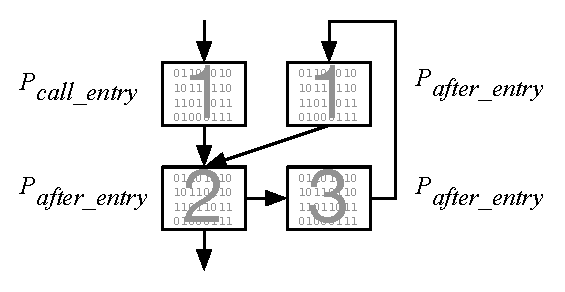
\epsfig{file=diagrams/policy-switching-entry-tracking.eps,width=2.5in}
\ORIGcaption{Instrumented Basic Blocks}
\end{subfigure}
\caption{\label{fig:policy_switching}Example policy switching protocol that ensures that instrumentation ($P_{call\_entry}$) is performed only once on entry to every function, regardless of if that basic block is re-executed. Basic block (1) is instrumented by both $P_{call\_entry}$ and $P_{after\_entry}$, and basic blocks (2) and (3) are instrumented by $P_{after\_entry}$.}
\end{figure*}


New module analysis tools are created by implementing one or more interacting instrumentation policies. Module analysis tools use policies to track state (called \emph{policy properties}) and decide how to instrument code.

Policies also serve a broader role in Granary itself. Granary maintains internal policy properties to optimise its performance and to track certain kinds of control flow. One example of a policy property used by Granary to optimise its user space performance is SIMD register tracking. When Granary detects the usage of a SIMD register, it sets the associated property. This property is inherited through the call chain, and informs Granary on whether or not the SIMD registers must be saved/restored when instrumented code yields to Granary. We say that an execution of a function $F$ is in the context of a usage of a SIMD register when the SIMD property is set. If $F$ is later executed by instrumented code where the SIMD property is not set, then a second instrumented version of $F$ (absent the SIMD property) will be stored in the code cache.

A developer prototyping a module analysis tool that uses multiple policies will automatically benefit from Granary's SIMD-tracking optimisation. Properties apply equally to all policies, and are inherited if/when a control-flow transfer effects a policy switch. However, not every control-flow transferring instruction (CTI) can explicitly change the policy used to instrument code: policies and their properties are not inherited across function returns. The motivation for this asymmetry is that conditions (e.g. SIMD register usage) present in a function $F$ might not be present in $F$'s caller. Because of this, function returns act as a natural mechanism for restoring instrumentation to a previous context. For example, Granary's SIMD register tracking is an effective optimisation because it limits the scope of saving/restoring the SIMD registers to only those yields performed in the context of a SIMD register, and not to all yields performed after the first usage of a SIMD register.

%.... set properties / properties naturally revert / etc. explain why no inheritance through RETs.

%This example of policy properties highlights some of their features: properties are inherited through control-flow instructions, even when policies themselves might change.

%Instrumentation policies are used to create new instrumentation tools and track state for those tools. An instrumentation policy is a set of functions that operate on a sequence of instructions ending in a non-call control-transfer instruction (CTI), called a basic block. The functions of a policy are responsible for adding instrumentation to a basic block and deciding what policy to apply to subsequent basic blocks. Granary is responsible for tracking and propagating any state associated with policies, called \emph{policy properties}.
%	
%	%State is tracked and propagated through the use of policy properties.
%	
%	%The functions of an instrumentation policy can arbitrarily manipulate the instructions of an instrumented program, as well as decide the ``next'' policy should be
%	
%	%Instrumentation policies are the means by which users of Granary can create instrumentation tools, as well as being the preferred mechanism for tracking and propagating state concerning the system's awareness of the code being instrumented.
%	
%	%Instrumentation policies in Granary serve two main purposes:
%	%\begin{inparaenum}[i)]
%	%	\item deciding how to instrument a sequence of instructions; and
%	%	\item tracking and propagating state/context using \emph{policy properties}.
%	%\end{inparaenum}

\subsection{Creating Tools with Policies}

Tool developers must implement three functions for each policy: \begin{enumerate}
	\item $F_{module}$ instruments a basic block of module code.
	\item $F_{kernel}$ instruments a basic block of kernel code.
	\item $F_{interrupt}$ handles an interrupt in instrumented code.
\end{enumerate}

The majority of tools will focus on implementing $F_{module}$; however, we have found $F_{kernel}$ useful when implementing \emph{data-driven instrumentation} and $F_{interupt}$ useful when implementing multiple weights of instrumentation in response to interrupt behaviour. 

%Granary provides a framework for fine-grained memory access instrumentation, called \emph{behavioural watchpoints}. Behavioural watchpoints-based tools expose tainted memory addresses to instrumented programs. If a tainted address is used to access memory then the processor raises a fault. Instead of instrumenting all code in a way that guards against such faults ($P_{watchpoints}$), Granary defaults to instrumenting basic blocks using $P_{null}$. However, when a fault is raised, Granary prevents future faults from occuring within the same basic block by patching the $P_{null}$-instrumented basic block to re-route control to a $P_{watchpoints}$-instrumented basic block.

For example, tools built with Granary's behavioural watchpoints framework expose tainted memory addresses to instrumented modules. Modules and the kernel freely share data, making it almost inevitable for  tainted addresses to ``leak'' into the kernel. If the kernel attempts to access the memory referenced by a tainted address then the processor will raise a fault. We handle this fault by applying $F_{kernel}$ to instrument the faulting kernel code using a policy that protects against such faults ($P_{watchpoints}$). $F_{interupt}$ is also used to optimise the execution of tools using behavioural watchpoints by initially assuming that code will not dereference a tainted address ($P_{null}$) and upgrading to $P_{watchpoints}$ if a fault on a tainted address occurs within a $P_{null}$-instrumented basic block.

% instrument as much or as little of the kernel as they want in response to this fault.
%Instrumentation policies expose three functions: one to instrument module code, one to instrument kernel code, and one to handle an interrupt in instrumented code.


$F_{module}$ and $F_{kernel}$ can abitrarily manipulate instructions and policy properties before they are packaged into basic blocks. These functions decide what the ``next'' policy should be for each CTI within the basic block. For example, if $P_{call\_entry}$'s $F_{module}$ sets the policy of a CTI in the basic block to policy $P_{after\_entry}$, then any module code targeted by the changed CTI will be translated and instrumented by $P_{after\_entry}$'s function $F_{module}$ (\Cref{fig:policy_switching}). 

%Because Granary depends on DynamoRIO's instruction encoder/decoder, the full range of DynamoRIO instruction/operand manipulation functions can be applied to instructions within a basic block.

\subsection{Managing State with Policies}

Policies encode state in the form of properties. A policy property describes an aspect of the environment in which the instructions of a basic block execute. Properties are tested, set, and unset by Granary and tool-specific policies over the course of decoding, instrumenting, and packaging instructions into basic blocks. By default, properties are propagated across all control-flow transfers except for return instructions. Property propagation through function call instructions enables inheritance of contextual information through the function call chain. The lack of propagation through function returns enables execution to return to a previous context.

Granary encodes policy information into the meta-data and CTIs of basic blocks. When an instrumented CTI executes for the first time, it yields control to Granary with the CTI target and policy information as inputs. Granary decodes and instruments the targeted instructions according to the input policy information. Granary depends on these inputs alone as a means of ensuring consistency: Granary cannot ``lose track'' of state concerning the execution of some code because the code itself maintains that state.  This enables arbitrary pre-emption and resumption of instrumented code without negatively affecting how as-of-yet uninstrumented code will be instrumented. The value of this approach is that it simplifies the process of creating instrumentation tools that run in OS kernels.

Granary's approach to managing state was motivated by our experience of trying to analyse modules with DRK. DRK maintains control over the execution of instrumented code by tracking what code is executing on each CPU. However, maintaining the consistency of this state is challenging: interrupts and exceptions introduce re-entrancy issues that are solved on a case-by-case basis. The complexities of managing the existing state increased when we modified DRK to only instrument modules and not the kernel. We found that our modified DRK sometimes ``got lost'' because of the interaction between interrupt handling, state management, and patching of translated code.

%We found that DRK sometimes ``got lost''  when analysing modules because the mechanism 
%because of the interaction of interrupt-handling, state-management, and patching of translated code.
%A property is set when Granary detects the usage of a SIMD register. This property is inherited through through the call chain.
%  The latter property is used by Granary to decide how to handle interrupts within instrumented kernel code.
%Instrumentated code can be arbitrarily pre-empted and resumed without concer.
%instrumented code yields control to Granary to build further basic blocks
%Granary was designed to operate in a multi-threaded, multi-core, pre-emptive kernel.
%Policy properties are encoded into the control-transfer instructions and meta-data of each basic block. This ensures that once emitted, the policy information of a basic block is immutable. 
%This is beneficial because Granary behaves in a purely functional way with respect to policies: 
%to be \emph{pure} with respect to policies: Granary's behaviour is fully-determined by 
%Policy properties are eventually immutable because they are directly encoded into the instructions and meta-data once 
%Policy properties are eventually immutable because once instructions have been packaged into a basic block, the properties that determined how those instructions, as well as any instructions targeted by control-transfer instructions within the basic block, were translated/instrumented never changes. 
%Immutability has the benefit of simplifying consistency when running in 
%that are tested, set, and unset by Granary and its policies during basic block creation.
%\paragraph{Policy behaviours}
%\paragraph{Policy conversions} can occur at any control-transfer instruction, with the exception of return instructions.
%If instrumentation purposefully exposes addresses that generate faults when accessed, then a policy interrupt handler can patch the original basic block to re-route control to a version of the original basic basic block that will guard itself against faults on memory accesses. This technique is used by Granary to optimise applications using \emph{behavioural watchpoints} to do fine-grained memory access instrumentation.
% TODO interrupts
%An example of how multiple policies are 
%Changing the policy during execution is useful for 
%\subsection{Clients}
%An instrumentation policy is a mechanism for deciding how to instrument a sequence of instructions, as well as how to instrument instructions targeted by any control-flow transferring instructions within the sequence.
%is a mechanism for maintaining and propagating immutable state that is used to decide how to instrument a sequence of instructions.
%is a mechanism for deciding how to instrument a sequence of instructions based on
% maintaining and propagating immutable state within a DBT system.
%and propagating state, as well as deciding how to instrument a sequence of instructions.
%\section{Managing State}\label{sec:state}
%Granary manages state using three mechanisms: shared data, CPU-private data, and instrumentation policies. 
%\paragraph{Shared data:} Granary maintains a centralised cache of all instrumented code, called the \emph{code cache}. The code cache is a data store that maps native (uninstrumented) code addresses to sequences of instrumented instructions, stored in the form of \emph{basic blocks} and their meta-data. 
%In Granary, a basic block is a maximal sequence of instructions that end in a non-function-call control-flow instruction. The inclusion of function calls within basic blocks is deliberate: Granary operates using a relaxed transparency model, and including function calls is a natural optimisation opportunity given this model. Addresses into the code cache are ``leaked'' to instrumented programs in the form of return addresses saved on the run-time call stack. Code cache addresses also leak to native code when mixed-mode execution is employed. Our experience with kernel instrumentation is that the kernel is not sensitive to such leaks. We have not yet encountered 
%\paragraph{CPU-private data:} Each core maintains a private mapping of native code addresses to code cache code addresses. This mapping
%When a new basic block is translated and stored in the global code cache, the mapping between the basic block and the nativ
%\paragraph{Instrumentation policies:}

\begin{figure*}[t!]
\lstset{language=C, tabsize=2, stepnumber=1}
\begin{multicols}{2}
\begin{lstlisting}[basicstyle=\footnotesize\ttfamily]
struct device_driver {
	...
	int (*probe)(struct device *);
	int (*remove)(struct device *);
	void (*shutdown)(struct device *);
	int (*suspend)(struct device *, pm_message_t);
	int (*resume)(struct device *);
	...
	const struct dev_pm_ops *pm;
	...
};
\end{lstlisting}
\columnbreak
\begin{lstlisting}[basicstyle=\footnotesize\ttfamily]
TYPE_WRAPPER(struct device_driver, {
    PRE_OUT {
        ABORT_IF_FUNCTION_IS_WRAPPED(arg.probe)
        WRAP_FUNCTION(arg.probe);
        WRAP_FUNCTION(arg.remove);
        ...
    }
    POST_OUT {
        POST_WRAP(arg.pm);
    }
})
\end{lstlisting}
\end{multicols}
\caption[LoF entry]{Example type wrapper for the Linux \texttt{device\_driver} structure. In the above code, \texttt{arg} is a reference to a \texttt{struct device\_driver} object passed as or referenced by an argument to a kernel or module function. Granary automatically applies type wrappers to function arguments passed over the kernel/module interface. Type wrappers are applied recursively (e.g. \texttt{POST\_WRAP}) up to a pre-defined depth. \texttt{PRE\_}, \texttt{POST\_}, and \texttt{RETURN\_} define wrapping policies applied before, after, or to the return value of a function used transfer control to/from the kernel or the module, respectively. The \texttt{\_IN} and \texttt{\_OUT} suffixes define the direction of data: \texttt{\_IN} wrappers apply to data going from the kernel into the module, and \texttt{\_OUT} wrappers apply to data leaving the module.}
\label{fig:type_wrapper}
\end{figure*}

\section{Mixed-Mode Execution}\label{sec:modes}
Granary supports two modes of execution: instrumented and native. Instrumented code runs under Granary's control and native code runs outside of Granary's control. Mode switches occur at well-defined \emph{attach} and \emph{detach} points. Detaching occurs when execution transfers from instrumented code to native code, and attaching occurs when execution transfers from native code to instrumented code. The benefit of mixed-mode execution is that tools can run some code (e.g. kernel code) without overhead by not instrumenting that code. This is valuable because module analysis tools can operate without negatively affecting the rest of the kernel's performance.

%The benefit of this feature is that tools have the option to run some code without overhead by not instrumenting that code. The value of this feature is that instrumentation tools can target and instrument specific code without negatively affecting overall system performance.\comment{!!!Qualify me!!!} Granary implements mixed-mode execution by relinquishing control at detach points and regaining control at attach points. This makes Granary \emph{comprehensive}: it controls/instruments all execution of any code of interest.

TODO TODO TODO: Describe the ``first attach'' by saying how Granary interposes on module initialisation.

\subsection{Detaching}

Granary detaches when control transfers from instrumented code to native (uninstrumented) code. If module code invokes a kernel function then the associated instrumented version of the module code will detach when the call executes. In this case, detaching is explicit because Granary knows that control will transfer to native code. Implicit detaches occur when instrumented module code returns to kernel code or is interrupted. Detaching is implicit in this case because instrumented module code does not know when it will be interrupted or if it was invoked by a kernel function (unless a tool tracks this using policies). 

% invoke a kernel \emph{function wrapper}.
%An explicit detach occurs when the translated version of module
%Instrumented module code implicitly detaches when it is interrupted or returns to kernel code, and explicitly detaches when module code that invokes a kernel function is translated to invoke a kernel \emph{function wrapper}.

Granary translates kernel function calls in module code into instrumented calls to kernel \emph{function wrappers}. A kernel function wrapper is an automatically generated intermediary function between instrumented modules and the kernel. Kernel function wrappers give Granary and its tools access to the arguments and return values of wrapped functions. Inspecting arguments and return values at the kernel/module boundary is safe because it is a point where modules (regardless of their internal programming) must follow the kernel ABI and agree on data structures.

Granary uses kernel function wrappers to actively find attach points. Attach points are exposed as function pointers stored in data structures that modules share with the kernel. For example, a device driver module registers itself with the kernel by sharing a pointer to a \texttt{struct device\_driver} object. This object contains several function pointers (e.g. \texttt{probe}, \texttt{remove}) back into the module's code. These function pointers represent attach points: if the kernel invokes one of the function pointers then Granary will take control. Granary finds these attach points and converts then into wrapped module functions. A wrapped module function is like a wrapped kernel functions in that it gives Granary and its tools access to the arguments/return values of an instrumented module function before and after that function is executed.

Granary uses \emph{type wrappers} to find and wrap module function pointers stored in shared data structures (\Cref{fig:type_wrapper}). A type wrapper defines functions that recursively  traverse the in-memory object graph and convert pointers to module code into pointers to wrapped module functions.  Granary automatically applies the correct type wrapper to each argument of a wrapped kernel/module function. 

We say that Granary ``bootstraps'' attaching on detaching because the data structures shared at detach points are used to discover new attach points.

%The net effect of argument and return value wrapping at detach points is to lazily discover attach points.
%of  is ``bootstrapped'' on detaching insofar as Granary lazily learns about attach points through the shared data structures of detach points.
% and is applied to each argumented to a wrapped kernel function.
%If the kernel directly invokes one of these function pointers then Granary is required to attach and instrument the invoked code.
%If the kernel were to directly invoke one of these function pointers then 
%when a device driver (a kind of module) registers itself with the kernel, it shares a \texttt{struct device\_driver} object 
%occurs when instrumented module code invokes a kernel function (explicit), returns to kernel code (implicit), or is interrupted (implicit). If module code invokes a kernel function, then the instrumented version of that module code will invoke a wrapped version of the kernel function. 
% Internally, Granary uses this ability to optimise re-attaching.
%Wrapped kernel functions are automatically created by Granary. They give Granary and its tools access to the arguments and return values of the functions being wrapped. Internally, Granary uses wrappers to inspect  function arguments and objects that they may reference in order to find function pointers leading back to uninstrumented module code.
%The effect of detaching is an implicit relinquishing of control: instrumented code directly transfers control to native kernel or to a wrapped kernel function. Granary creates small copies of every kernel function, called kernel wrappers, that invoke the original kernel functions. 

\subsection{Attaching}
Attaching occurs in one of three ways: \begin{enumerate}
	\item {\bf Implicit attaching:} the kernel returns to instrumented module code.
	\item {\bf Fast attaching:} the kernel invokes a wrapped module function.
	\item {\bf Slow attaching:} the kernel invokes unwrapped module code. Granary uses memory page protection to mark the code of modules-to-be-instrumented as non-executable. Making module code non-executable helps Granary ensure comprehensiveness: if the kernel finds an ``alternate route'' to invoking module code then the processor will refuse to execute that code and instead raise a fault. Granary handles this fault by returning execution to the instrumented version of the faulting module code.
\end{enumerate}

Fast and slow attaching transfer control instrumented module code. Fast attaching is ``fast'' because the instrumented code address is computed once and emitted as part of the module function wrapper. Slow attaching is ``slow'' because Granary looks up the instrumented address associated with the faulting native address each time the fault occurs.

\subsection{Transparency}\label{sec:transparency}
An instrumentation system is transparent if the instrumented and uninstrumented versions of a program behave in the same way given the same inputs \cite{Transparency}. By default, Granary operates under a relaxed transparency model: certain artifacts of Granary existence (e.g. instrumented code addresses, changes in timing) are exposed to the kernel and to instrumented modules. Some artifacts are unavoidable. For example, instrumented code (typically) executes more slowly than native code because of additional indirection added by Granary. Granary also requires memory to operate---memory that once allocated becomes unavailable for other uses. Some artifacts that break transparency can be avoided; however, the mechanisms required to maintain transparency in these cases introduce additional overheads.

The trade-off between transparency and overhead motivated the inclusion of configurable levels of transparency in Granary. Granary defaults to being non-transparent for efficiency and flexibility, and if transparency is needed to instrument a module then transparency can be enabled at the cost of increased overheads. By default, Granary exposes the following artifacts: \begin{enumerate}
	\item Instrumented code addresses as return addresses in function activation frames.
	\item Instrumented code addresses as return addresses in interrupt stack frames.
	\item Wrapped module function addresses in shared data structures.
\end{enumerate}

%Our experience is that most modules are not sensitive to the ways in which Granary is not transparent.
% Granary is not fully transparent because it exposes instrumented code addresses to the kernel and to instrumented modules.
%If an instrumentation systems ensures that instrumented programs behave exactly and uninstrumented programs then they ar
%If an instrumentation system risks changing the instrumented program's behaviour then the system is not transparent. Granary 
%Implicit and fast attaching are achieved by exposing instrumented code addresses to the kernel and its modules. Instrumented code addresses are exposed as return addresses in function activation frames and interrupt stack frames, and as wrapped module function addresses in shared data structures. Exposing these addresses risks altering the module's behaviour: some modules might depend on specific return address values or function pointer values (stored in a shared data structure). 
%The following list describes the ways in which Granary is and is not transparent:

\paragraph{Function return addresses} By default, Granary does not maintain return address transparency. Return addresses to instrumented code are exposed to instrumented functions and kernel functions. The benefit of not maintaining return address transparency is efficiency: Granary will not do extra work (i.e. an indirect branch lookup) to resolve the target of a \texttt{ret} (return from procedure) instruction. If Granary is configured to use transparent return addresses, then implicit attaching and detaching are disabled. Granary will fall back to depending on slow attaching and performing an indirect branch lookup before executing \texttt{ret} instructions.

\paragraph{Interrupt return addresses} Kernel interrupts are not sensitive to return addresses, except in the case of page faults occuring within specific kernel functions that access user space data. Therefore, maintaining return address transparency with respect to interrupts in instrumented module code has no value. Granary treats faults in kernel code that accesses user space data as a special case and handles those kinds of interrupts in a similar way to the kernel.

%The benefit of this approach is that interrupts are never delayed, unless explicitly requested by tool developers.  Our experience with writing module analysis tools using DRK motivated Granary's lack of interrupt return address transparency. DRK-based analysis tools that want to maintain transparency are restricted by DRK's approach to handling interrupts. DRK limits tools to 

\paragraph{Module function wrappers} Granary does not maintain transparency when its type wrappers replace pointers to module functions with pointers to wrapped module functions. This is perhaps the riskiest break in transparency within Granary because a module might treat a function pointer as being representative of the module being in some particular state. The benefit of enabling module function wrappers is that they give instrumentation tools more information about the executing module (e.g. shared data structures, which interfaces are used by the kernel). If Granary is configured to use transparent module function pointer addresses in shared data structures then fast attaching is disabled and tools will not have access to the same level of static program information.



%We intend to extend Granary to instrument all kernel code. 

%Typical kernel modules are written in C and sometimes mixed with assembly. There is good motivation for writing modules in C: the Linux kernel has many useful macros and inline functions that aren't directly available to assembly. To the best of our knowledge, C compilers do no

%\begin{enumerate}
%	\item {\bf Function return addresses:} Instrumented module functions and kernel functions can 
%	\item {\bf Interrupt return address:}
%	\item {\bf Data structure function pointers:}
%	\item {\bf Stack pointer:} 
%\end{enumerate}


%values of a function's return address or function pointer 
% function return addresses or 
%A detach point is any kernel code called by instrumented module code. An attach point is module code that is 
%A detach point is any kernel function and an attach point is any module code executed by the kernel. Granary statically analyses the kernel source code to learn about detach points and their specifications. Granary dynamically ``learns'' about attach points by observing module code addresses as they cross the module/kernel interface. A typed attach point is a
% in the form of shared function pointers. Granary detects shared function pointers by recursively inspecting the data passed over the kernel/module interface using type wrappers (\Cref{fig:type_wrapper}).



%Granary enables instrumentation tools to blah blah blah.

\section{Reifying Instrumentation}\label{sec:reify}

Existing program analysis systems fall into one of three categories:
\begin{enumerate}
	\item Binary analysis tools. Existing tools give low-level access to instructions and possibly memory but don't give ``big-picture'' information available source code analysis tools \cite{DRK,DynamoRIO,Pin,PinOS,QEMU,Valgrind}.
	\item Source code analysis tools. Existing tools give high-level access to program semantics but make it challenging to reason about scheduling, interrupts, shared memory, and aliasing [TODO: cite Sparse, Smatch].
	\item Mixed source/binary analysis tools. Existing tools give high- and low-level access to program informaiton, but require changes to the compilation toolchain and sometimes program source code \cite{NaCl,AddressSanitizer,ThreadSanitizer}.
\end{enumerate}

The benefits of high-level static analysis information motivated its inclusion into Granary using a technique we call reifying instrumentation. Granary extracts type and function declarations from the Linux kernel source code and exposes that information to tool developers. Because of this, tools can inspect data at mode-switch boundaries (kernel and module wrappers) and dynamically change the instrumentation policy based on type information.

We say that static type information is \emph{reified} because Granary re-introduces it into module binaries by using it to discover attach and detach points. Type information reified by Granary can guide runtime instrumentation decisions. For example, a tool can switch the instrumentation policy based on memory accesses to data of a particular type or based on the usage of a particular module/kernel interface. Tools can also dynamically learn the runtime types of module-allocated objects by observing pointers to those objects as they cross the module/kernel interface.

%Granary \emph{reifies} static type information by using it to guide attaching and detaching, as well as by allowing tools to base runtime instrumentation decisions 
%
%re-introducing it into ``typeless'' module binaries.  Granary understands the module/kernel boundary using attach (kernel wrappers) and detach (module wrappers) points.
%
%at the module/kernel boundary
%
%We call the technique of using static analysis information in Granary ``reifying instrumentation'' because:
%\begin{enumerate}
%	\item Static type information is not present in module binaries. Granary re-introduces type information into ``typeless'' module binaries because modules use kernel functions and data structures to interact with the kernel.
%	\item Static program information can guide runtime instrumentation decisions. For example, the policy used to instrument code can be changed based on:
%	\begin{enumerate}
%		\item A memory access to data of a particular type.
%		\item The usage of a particular interface (kernel function or function pointer field within a kernel data structure).
%		\item The presence of an object of a particular type being passed as an argument to a module function.
%	\end{enumerate}
%	\item Runtime type information can be dynamically learned. For example, if a module allocates some memory then that memory is initially typeless. However, if a Granary tool observes that the allocated object is reachable from an argument to a module or kernel function wrapper then a type can be assigned to that memory.
%\end{enumerate}



We are actively developing a tool that uses reifying instrumentation to create models of module behaviour. Reifying instrumentation serves two roles in this tool. First, we use type information known at mode-switch boundaries to assign kernel types to module allocated memory that is shared across the module/kernel interface. Type assignment plays a critical role because it allows us to correlate memory reads and writes within an object to the exact structure fields of that object. Second, we use the kernel and module function wrappers to generate compressed call graphs of a module's execution from the perspective of the kernel.  When combined, this information allows us to say when and where specific parts of kernel data structures are accessed and modified. Finally, we combine the information recorded from executing multiple ``trusted'' modules (e.g. mature, open-source file systems) and construct models of typical module behaviour. We hope that these models will help us to automatically generate new tools that identify spurious module behaviour.


%By combining this information from multiple ``trusted'' modules (e.g. mature, open-source file systems), we hope to be able to create instrumentation that discovers spurious module behaviour 

%For example, we can use the static information available to Granary to create a tool that generates code that, when executed, checks that it is 

%kernel and module wrappers can be combined with policy-switching to enforce some API usage integrity constraints. For example, policy switching can be used to accept or reject an execution of module code by observ

%most useful at mode-switching boundaries, where 

%Static program information is available to Granary tools in the form of kernel types and function declarations. Tools can operate on this information with meta-programs, as well as observe 

%Tools can use this information to interface with the kernel or to 

%We use this information in several novel ways:
%\begin{enumerate}
%	\item 
%\end{enumerate}

%Tools can use meta-programs to operate on this information and generate code (at the tool's compile time) that coordinates with the tool's dynamic analyses in order to learn more about module code. 

%This technique, which we call ``reifying instrumentation'', is distinct from typical dynamic analysis
%We call the technique of mixing static program information into a DBT system ``reifying instrumentation'' because it takes abstract information (e.g. type information) which is absent from module binaries and re-introduces it as actionable data. This data is actionable insofar as the 

%Granary exposes static program information to instrumentation tools in the form of 
%Granary tools can use static program information 
%Reifying instrumentation is the process of using static program information known at mode-switch boundaries to guide the application of different instrumentation policies. The key insight of reifying instrumentation is that the execution of attach and detach points (kernel wrappers) give clues as to how modules and the kernel are interacting.
%Reifying instrumentation allows tools to inspect and manipulate a portion of program memory at attach (module wrappers) and detach points and in a well-defined way. 
%This is useful because it helps the instrumentation system learn more about the execution of an otherwise opaque binary. The value of this feature is that users can create low-level instrumentation tools that operate on programs in a high-level way. 
%Granary uses a technique that we call reifying instrumentation in order to 
%The key insight of reifying instrumentation is that even arbitrary binaries must follow conventions and APIs to correctly interact with other programs.
%\section{Environment}\label{sec:env}
%\subsection{Interrupts and Exceptions}\label{sec:interrupts}

\section{Evaluation}\label{sec:eval}
Granary is designed to comprehensively instrument kernel modules. We first evaluated the performance of Granary framework alone by running it with different kernel modules. We ran the experiment on a desktop equipped with an Intel\textregistered\ Core\texttrademark\ 2 Duo 2.93 GHz CPU, 4GB memory, and an Intel 82598EB 10 Gigabit Ethernet controller. We used IOzone filesystem benchmark to exercise ext3 module while running it with Granary. Iozone is a useful benchmark for testing data throughput with number of different access pattern. we avoided bottleneck for disk I/O by partitioning main memory to load ext3 module. To compare the throughput of Granary with existing kernel instrumentation framework, we modified DRK to instrument only kernel modules. We implemented similar attach/detach mechanism for DRK at module interface. The framework uses similar kernel wrappers for fast attach and page protection as fall back mechanism to gain control. For initial evaluation of Granary, we developed null policy client and enabled wrap depth optimization by limiting it to 2.


\begin{table*}[thp!]
\caption{Iozone Throughput for different filesystem operations}
% title of Table
\centering
% used for centering table
\begin{tabular}{c c c c}
% centered columns (4 columns)
\hline\hline
%inserts double horizontal lines
Workload & Native & Granary & Modified DRK  \\ [0.5ex]
% inserts table
%heading
\hline
% inserts single horizontal line
Write & 184669.69 & 152223.03 & 55134.09 \\
% inserting body of the table
Read & 1577591.69 & 1648645.02 & 1421037.96 \\
Random Write  & 552380.48 & 412069.48 & 162847.34 \\
Random Read & 1644573.29 & 1597321.54 & 1636472.14 \\

Mixed Workload & 1168804.11 & 929383.54 & 915196.76 \\[1ex]
% [1ex] adds vertical space
\hline
%inserts single line
\end{tabular}
\label{table:nonlin}
% is used to refer this table in the text
\end{table*}

%wrapping mechanism for DRK to attach and detach the framework at module interface.

%and jbd modules while running them under Granary.   


%To evaluate our system with existing kernel instrumentation framework, we modified DRK to instrument only kernel modules. We implemented similar wrapping mechanism for DRK to attach and detach the framework at module interface. We checked the correctness of our system by running different filesystem and network modules(ext2/ext3, xfs, e1000e etc) under their control. To stress test the filesystem modules we used filesystem benchmark IOzone and ran the modules with null instrumentation client. null instrumentation client was used to avoid the overhead of instrumentation. We ran our tests on a desktop equipped with an Intel\textregistered\ Core\texttrademark\ i7-860 2.80 GHz CPU, 8GB memory, and an Intel 82578DM Gigabit Ethernet card.  

\section{Related Work}\label{sec:related}
TODO


\section{Conclusion}\label{sec:conclusion}

TODO
%\section{}\label{sec:

%\section{Architecture and Design}\label{sec:arch}

%In this section, we describe how Granary meets the goals laid out in \Cref{sec:goals}. To do so, we describe several challenges, alternative approaches, and the solutions we chose.

%Non-module kernel code executes without overhead when Granary instruments kernel modules using mixed-mode instrumentation.

%. First, if a module's code is meant to be instrumented, 

%, both with respect to ensuring that no module code escapes instrumentation, and 

%The environment in which the kernel and its modules execute introduces 
%Often the environment in which kernel and module code executes obfuscates the 
% and the Linux kernel and its modules execute in a complex and dynamic environment. To ease development of new tools, Granary was designed to instrument user space programs in Linux and Mac OS X.
% to have zero overhead, while also allowing further type, policy, and argument manipulation at the point when Granary regains control.
%Granary enables users to interpose on and alter the behaviour 
%at mode-switch boundaries  in a type-safe way
%propagating this information deeper into an otherwise opaque binary.
%of using static program information (type information, semantic information) to guide the choice of which instrumentation policy to apply at attach points, as well as to propagating this information from attach and detach points into an otherwise opaque binary.
%Mixed-mode execution is challenging to implement because Granary is \emph{comprehensive}: the execution of any code of interest is always controlled by Granary. 
%A DBT system is \emph{comprehensive} if it controls/instruments all execution of any code of interest. 
%Mixed-mode execution is challenging to implement because Granary must relinquish its control at a detach point, but (efficiently) regain control at an attach point.
%Mixed-mode execution is challenging to implement because it requires that a DBT system relinquishes its control at a detach point, but has a mechanism to (efficiently) regain control at an attach point. If a DBT system can ensure that it controls/instruments all code of interest, then it is \emph{comprehensive}. Granary solves the problem of comprehensiveness in the face of mode switches using three techniques: static wrappers, dynamic wrappers, and page protection.
%Mixed-mode execution is implemented by relinquishing control at detach points, and regaining control at attach points. The key challenge of implementing mixed-mode execution is how to (efficiently) regain control once it has been relinquished. If a DBT system can ensure that it controls/instruments all code of interest, then it is \emph{comprehensive}. Granary solves the problem of comprehensiveness in the face of mode switches using a combination of \emph{static wrappers}, \emph{dynamic wrappers}, and page protection.
%If a DBT system ensures that all code of interest is instrumented
%users are not required to pay the overhead of the DBT system on code that they are not interested in instrumenting. 
%However, implementing mixed-mode execution is challenging. If a DBT system relinquishes its control over a program's execution, then there is no guarantee that the DBT system will regain control before code to be instrumented is next executed. A DBT system is \emph{comprehensive} if it ensures that all code of interest is instrumented, regardless of if execution control is relinquished. Granary solves the problem of comprehensiveness in the face of mode switches using a combination of \emph{static wrappers}, \emph{dynamic wrappers}, and page protection.
%---in order to comprehensively instrument code of interest (e.g. a kernel module)---Granary must have a mechanism of regaining control even when a mode-switch from instrumented to native code \emph{relinquishes} its control.
%The key challenge of implementing mixed-mode execution is that of \emph{comprehensiveness} in the face of losing control. For example, Linux kernel module code ...
%The motivation for mixed-mode instrumentation is that a user should only have to pay the overhead of instrumenting code of interest. 
%The motivation for mixed-mode instrumentation is that one should only have to pay the cost of instrumentation for the code that one wants to instrument.
%focus on instrumenting that code which they care about.
%when to save those registers lest Granary accidentally clobber those registers and change the instrumented program's behaviour.
%Granary was originally developed as an extension to the DynamoRIO Kernel (DRK) \cite{Feiner2012} DBT framework; however, due to 
%While designing Granary, we identified four goals for efficient kernel instrumentation:
%\begin{enumerate}
%	\item {\bf Efficiency:} 
%\end{enumerate}
%Granary's key novelty is its pervasive support for \emph{mixed-mode execution}: the ability to switch between native and instrumented code on the fly. 
%, which allows users to focus on instrumenting 
%Due to its support for mixed-mode execution, Granary supports multiple granularities of instrumentation: function-, module-, kernel-, data-, and context-specific.
%Granary's key novelty is its ability to instrument a program at multiple granularities.
%\begin{itemize}
%	\item {\bf Function-specific:}
%	\item {\bf Module-specific:}
%	\item {\bf Kernel-specific:}
%	\item {\bf Data-specific:}
%	\item {\bf Context-specific:}
%\end{itemize}
%\section{Design}
%\subsection{Goals}
%Granary was originally designed for analysing Linux kernel modules. During Granary's design, we identified the following four goals: 
%\begin{enumerate}
%	\item[i)] Comprehensively analyse \emph{all} kernel modules.
%	\item[ii)] Impose no performance overheads on non-module kernel code.
%	\item[iii)] Require no changes to modules and minimal changes to the kernel.
%	\item[iv)] Be easily portable between different hardware and kernel versions.
%\end{enumerate}
%Prior work based on source code analysis and annotations \cite{YMao2011} fails to meet goals (i) and (iii), while work based on special hardware features or virtualization \cite{Xiong2011} fails to meet goals (i) and (iv), and work based on whole-OS or -system instrumentation/emulation \cite{Feiner2012} fails to meet goal (ii).
%\subsection{Mixed-mode Execution}
%Executing code belongs to one of three contexts:
%\begin{enumerate}
%	\item {\bf Host}: \texttt{libc} in user space, and the Linux kernel in kernel space. By default, code from this context executes at full speed and without interference from Granary. However, host code is sometimes instrumented depending on the configuration of the active \emph{instrumentation policies}.
%	\item {\bf Application}: Non-\texttt{libc} code in user space, and kernel modules in kernel space. By default, code from this context is instrumented according to one or more \emph{instrumentation policies}.
%	\item {\bf Granary}: Granary's runtime system manages host and application code.
%\end{enumerate}
%Granary is responsible for ensuring comprehensiveness with respect to an execution context. For example, if Granary is configured to instrument a particular kernel module, then Granary ensures that the execution....


\bibliographystyle{acm}
\bibliography{library}
\end{document}
